\begin{frame}{Birdclef CSE145/237d Team}
    \begin{itemize}
        \item Ludwig
        \item Geelon (5th year PHD)
        \item Sean O Brien(1st Year PHD)
        \item Vibhuti (3rd year CSE)
        \item Current Objective Literature Review
        \item Some inital ideas to explore 
    \end{itemize}
\end{frame}

\begin{frame}{Jacob's Work}
    \centering
    Problem:\\
    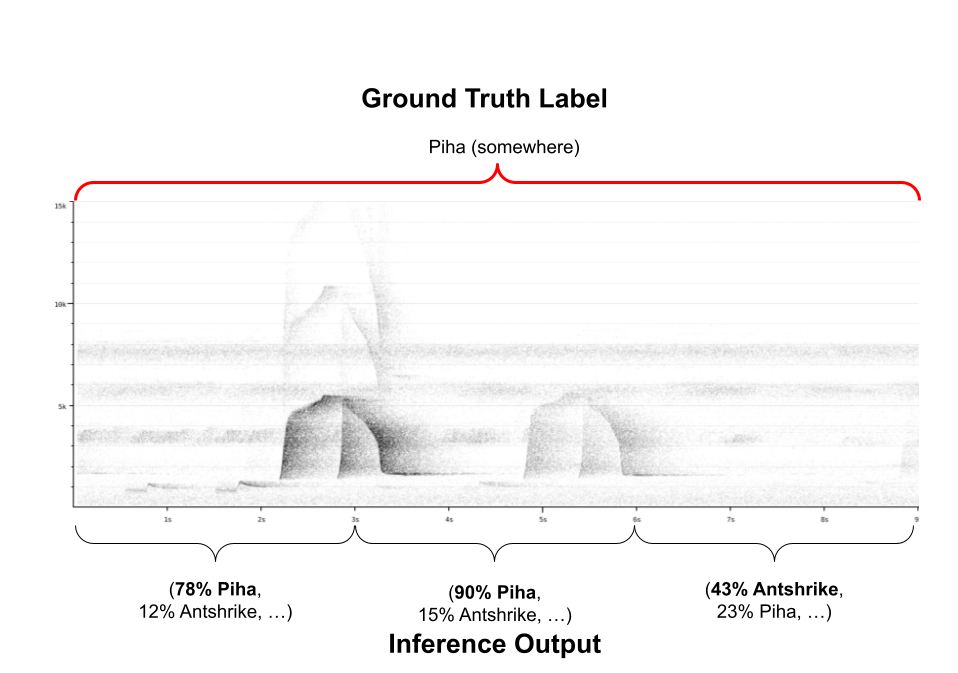
\includegraphics[height=0.9\textheight,width=0.7\textwidth,keepaspectratio]{images/spectrogram-.png}
\end{frame}

\begin{frame}{One Approach: Aggregation}
    \begin{itemize}
        \item Aggregate probabilities for chunks
        \item Max = label
    \end{itemize}
\end{frame}

\begin{frame}{One Approach: Aggregation}
    \centering
    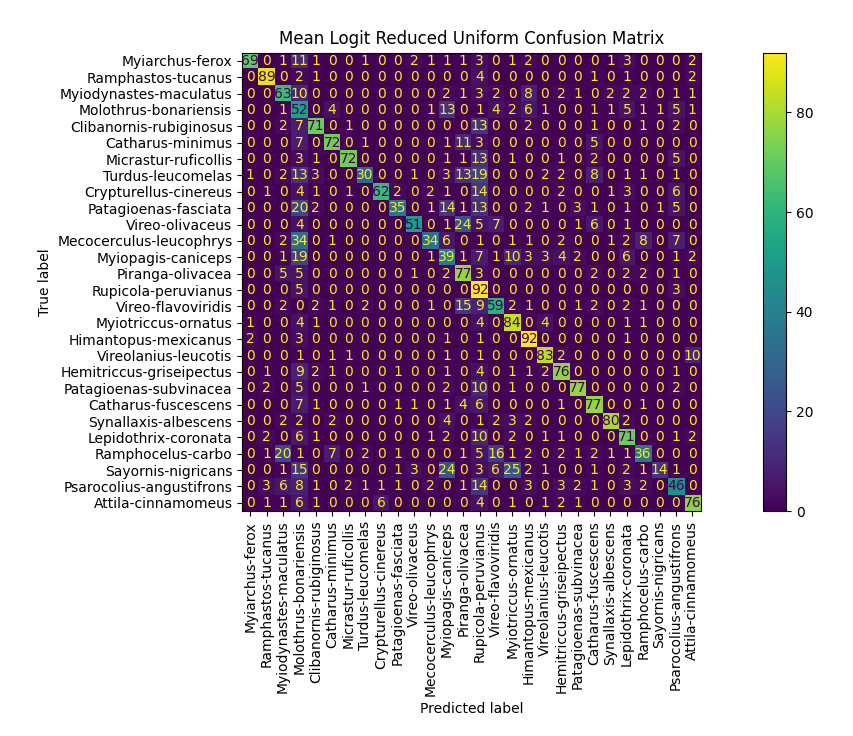
\includegraphics[height=0.8\textheight,width=0.7\textwidth,keepaspectratio]{images/logit_confusion_matrix.png}
\end{frame}

\begin{frame}{Multiple Instance Learning}
    \begin{itemize}
        \item "Bag" of labels for each clip
    \end{itemize}
    Analogy:\\
    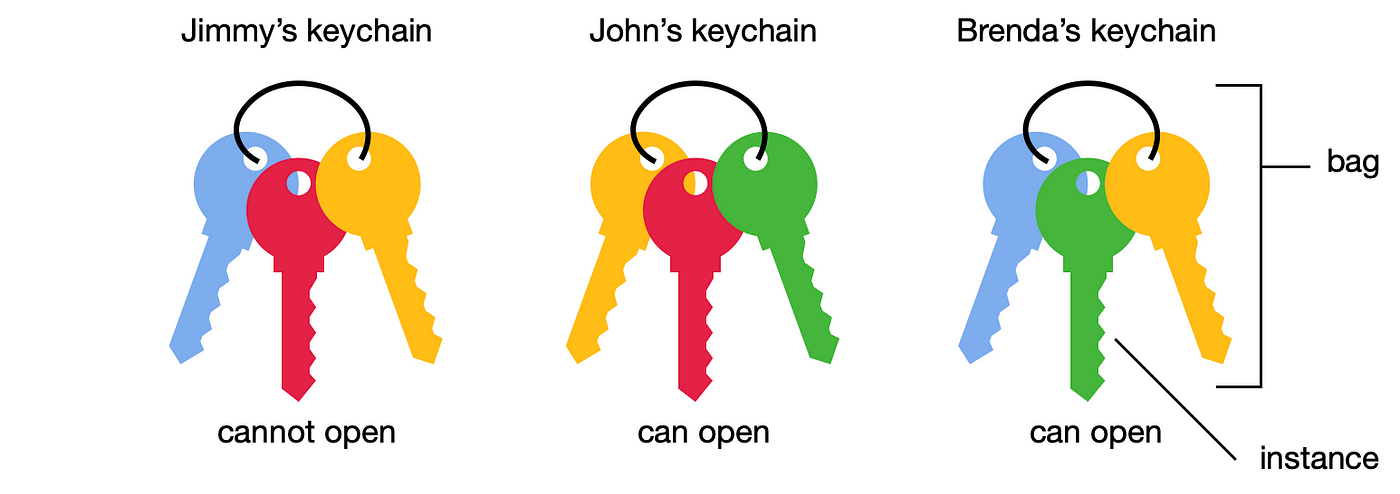
\includegraphics[height=0.7\textheight,width=0.7\textwidth,keepaspectratio]{images/keyring_analogy.png}
\end{frame}

\begin{frame}{Multiple Instance Learning}
    \begin{columns}
        \begin{column}{0.5\textwidth}
            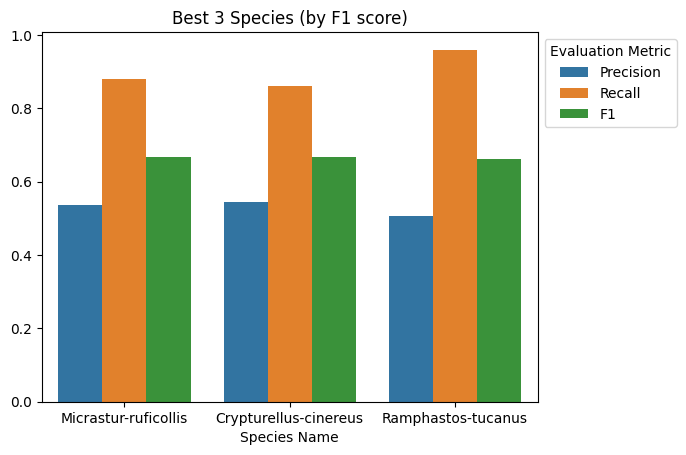
\includegraphics[height=1\textheight,width=0.7\textwidth,keepaspectratio]{images/best3species.png}
        \end{column}
        \begin{column}{0.5\textwidth}
            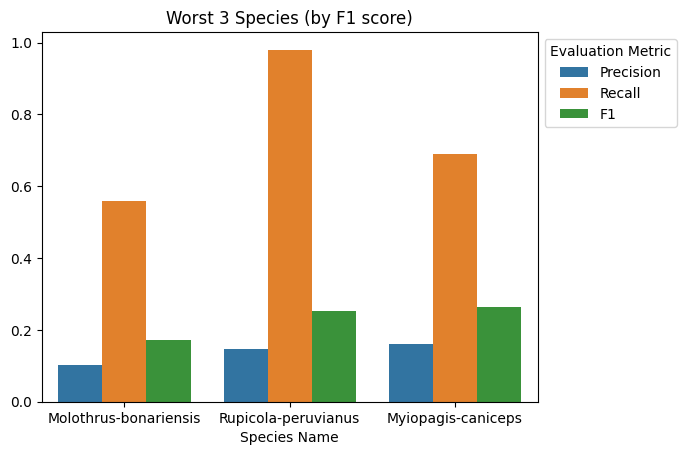
\includegraphics[height=1\textheight,width=0.7\textwidth,keepaspectratio]{images/worst3species.png}
        \end{column}
    \end{columns}
    \begin{itemize}
        \item High recall for both ends
    \end{itemize}
\end{frame}

\begin{frame}{Publication with Jacob}
    \begin{itemize}
        \item Local machine setup
        \item Kastner ML setup
        \item Timeline for this quarter
    \end{itemize}
\end{frame}

\begin{frame}{Google Cloud}
    \begin{itemize}
        \item 1,600 a month?
        \item 800 per instance
        \item Assumes same performance as aws
        \item Takeaway: AWS seems cheaper
    \end{itemize}
\end{frame}

% Slides for 2024-04-12
% To create a slide, use the following:
% \begin{frame}{TITLE}
%     BODY
% \end{frame}

% To create a slide with a bullet list, use the following:
% \begin{frame}{TITLE}
%     \begin{itemize}
%         \item ITEM 1
%         \item ITEM 2
%     \end{itemize}    
% \end{frame}

% To create a slide with numbered list, use the following:
% \begin{frame}{TITLE}
%     \begin{enumerate}
%         \item ITEM 1
%         \item ITEM 2
%     \end{enumerate}
% \end{frame}

% To create a slide with a graphic:
% 1. Add the graphic to this folder (named picture.png)
% 2. Use the following:
% \begin{frame}{TITLE}
%     \centering
%     \includegraphics[height=0.7\textheight,width=0.7\textwidth,keepaspectratio]{picture.png}
% \end{frame}

% To create a slide with two columns, use the following:
% \begin{frame}{TITLE}
%     \begin{columns}
%         \begin{column}{0.5\textwidth}
%             COLUMN 1 BODY
%         \end{column}
%         \begin{column}{0.5\textwidth}
%             COLUMN 2 BODY
%         \end{column}
%     \end{columns}
% \end{frame}
